\documentclass{article}


\usepackage[margin=1in]{geometry}
\usepackage{amsmath}
\usepackage{graphicx}
\usepackage{tabu}
\usepackage{float}
\usepackage{listings}
\usepackage{color}
\usepackage{caption}

\author{Zachary Vogel\quad Chuyi Liu}
\title{Real Time Embedded Exercise 2\\ ECEN 5623}
\date{\today}

\begin{document}





\maketitle

\captionsetup{labelformat=empty}
\section*{Problem 1}
To prove that we did in fact make an account on the DE1 board, We have this screenshot of a login on the board through Putty. The groups command as well as the whoami command illustrate that the account is in fact created.
\begin{figure}[H]
    \centering
    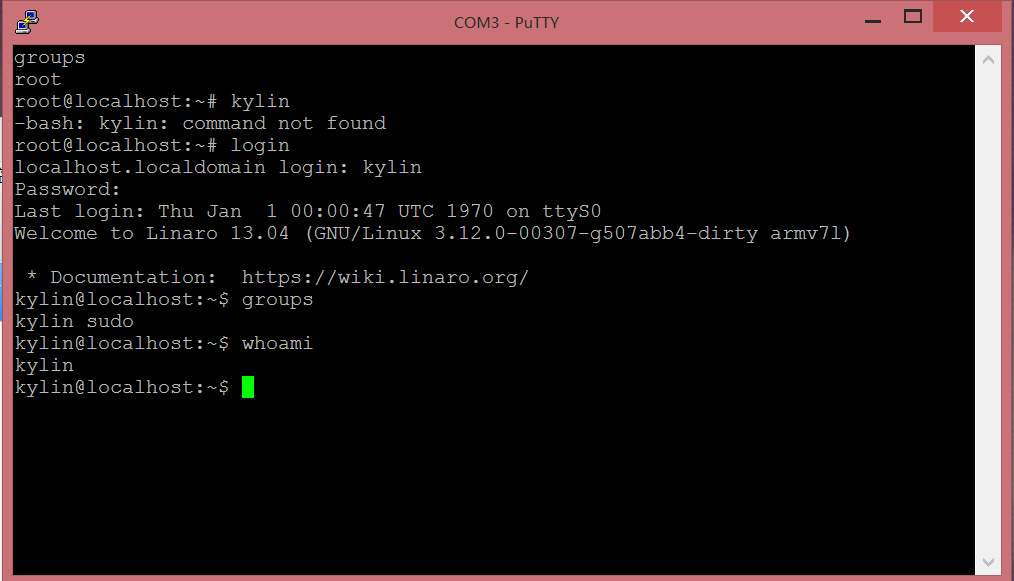
\includegraphics[width=0.8\textwidth]{p1.png}
    \caption{You can see the login as well as the account confirmation with whoami}
\end{figure}
\section*{Problem 2}
\subsection*{Explanation and Critique}
Within the frequency executive architecture, off-line processors are applied to compute data and provide a scheduling table. The high-frequency executive is scheduled at a higher priority compared to mid-frequency and low-frequency executive. That is similar to RM scheduling, which helps to ensure the feasibility and safety of the system. It may be applied to ensure all processing is completed in an extremely short time, which is good for systems that have high safety requirements[advantage-1].
Hence, this architecture is very helpful in guidance, navigation, and control(GN\&C) software, which performs a wide variety of functions with extremely tight timing and phasing relationships, the execution rates for its principal functions within an unique operation sequence(OPS) vary from 25 to 0.25 Hz.
This executive architecture is table-driven, its scheduling method is very deterministic, thus the executives are very simple and repeatable[advantage-2] compared to real-time software system. And thanks to which the system is more predictable[advantage-3] as long as overruns don?t occur. However, the table is not very flexible, we will have to recompute then change the whole table to make a little change, while in a real-time software system we don?t need to do that, for other words, it?s much harder to implement additional functions or requirements[disadvantage-1].
PASS uses eight different phase/function combinations, and each OPS has  different parts, modes, and thus substructures are implemented(like man/machine interface structure). This hierarchical structure makes the computation for the architecture more complex than for a real-time system. Due to the complexity, it requires a lot of off-line computation, which relays on off-line processors[disadvantage-2].
To make a successful implementation of PASS software, the system is supposed to pursue the implementation of software requirements in a top-down sequence and follow a release plan that used a building-blocking approach. Hence, tasks are supposed to have fixed release times[disadvantage-3].

\section*{Problem 3}
\subsection*{Coding}
We wrote a scheduler for LLF and EDF. We don't think they work because they pass tests that failed in cheddar, specifically sim 6 and 8 for LLF. We have no idea why, we spent hours debugging with no success. As far as we can tell the implementation gives the correct output. There are some print statements to give the output if you want to check, but they all seem to follow the rules. The only other thing that mgiht be causing a problem is setting the Deadline time to the LCM when computation
time is reset. The code is attached with a makefile. We also did a deadline utilization function, which similarly to
the RM LUB, won't pass any task sets that aren't feasible. It will fail some tests that are though. Both schedulers use the same idea, find min deadline or laxity, decrement computation time, always decrement the time to deadline, exit when the remaining computation is greater than deadline time, and reset on period. In that order specifically.\\

As for the feasibility tests, we could not determine a simple computation that gave a necessary and sufficient answer to the scheduling problem. We would be interested in seeing how Cheddar does this because most of the papers we read did not give a feasibility test outside of pure scheduling. Cheddar seems to do some calculation of worst case execution time, but it doesn't seem trivial to calculate.
\subsection*{Cheddar Conformation}
Here we have all of the output from cheddar for the various problems.
\subsubsection*{Example 4}
\begin{figure}[H]
    \centering
    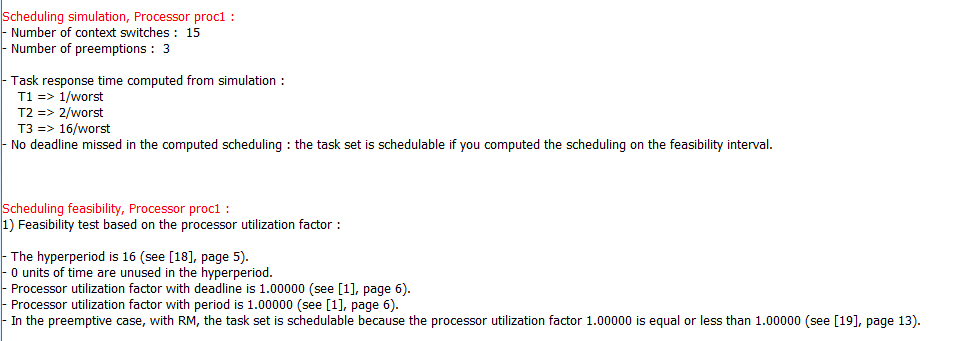
\includegraphics[width=0.8\textwidth]{4_RM.png}
    \caption{Example 4 Rate Monotonic}
\end{figure}
\begin{figure}[H]
    \centering
    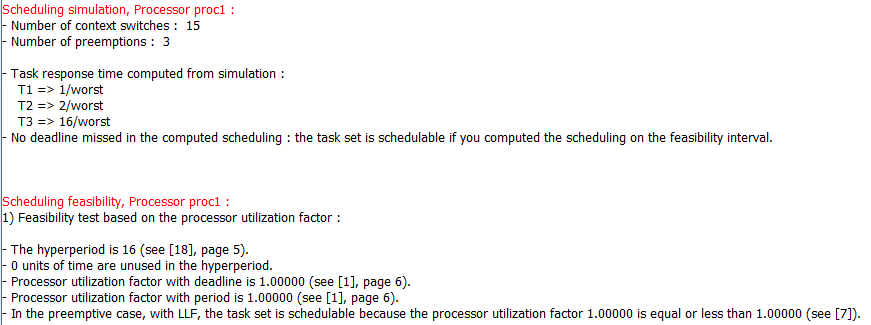
\includegraphics[width=0.8\textwidth]{4_LLF.png}
    \caption{Example 4 Least Laxity First}
\end{figure}
\begin{figure}[H]
    \centering
    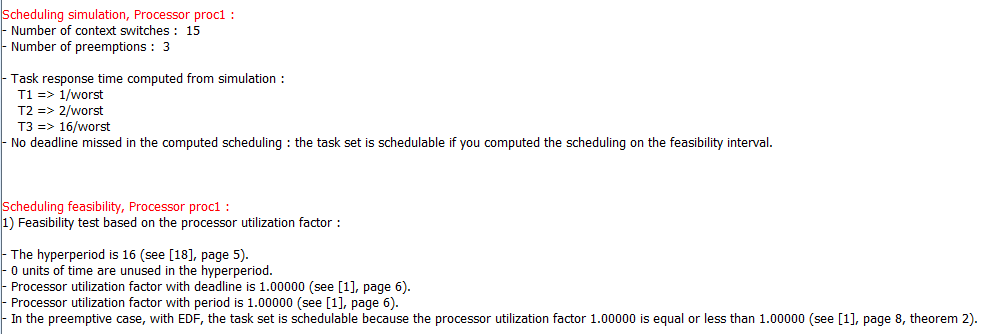
\includegraphics[width=0.8\textwidth]{4_EDF.png}
    \caption{Example 4 Earliest Deadline First}
\end{figure}

\subsubsection*{Example 5}
\begin{figure}[H]
    \centering
    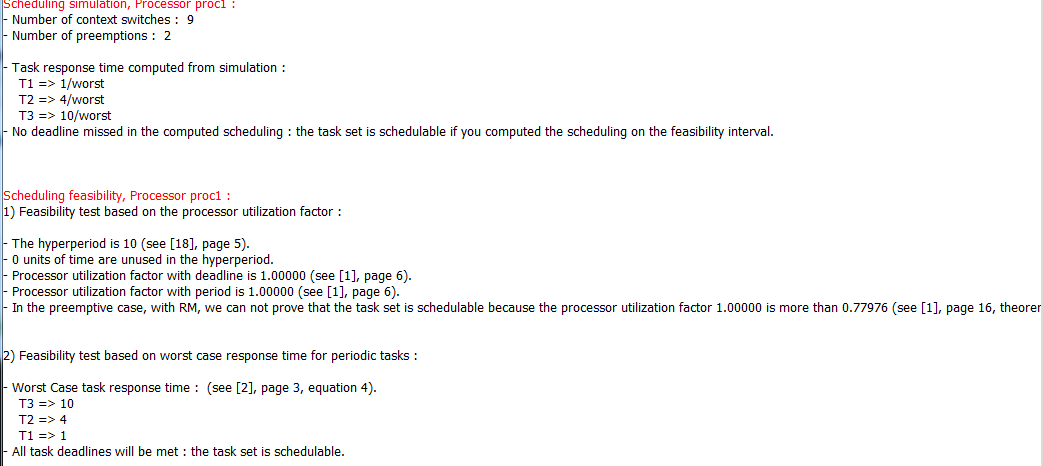
\includegraphics[width=0.8\textwidth]{5_RM.png}
    \caption{Example 5 Rate Monotonic}
\end{figure}
\begin{figure}[H]
    \centering
    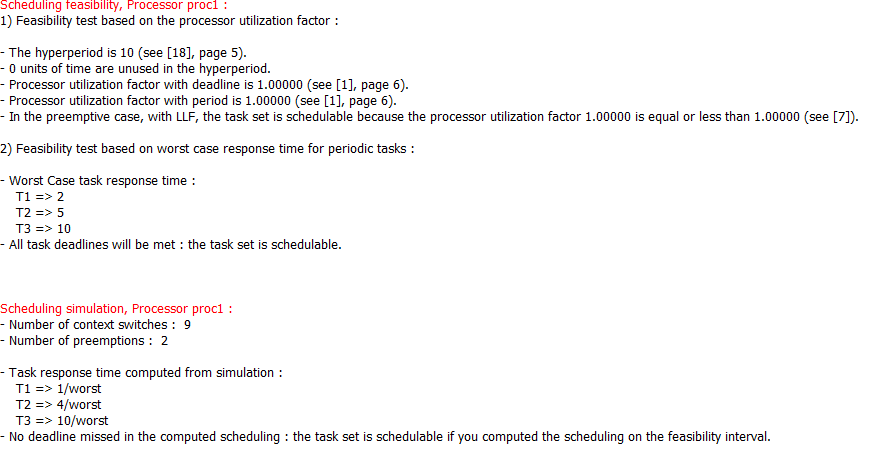
\includegraphics[width=0.8\textwidth]{5_LLF.png}
    \caption{Example 5 Least Laxity First}
\end{figure}
\begin{figure}[H]
    \centering
    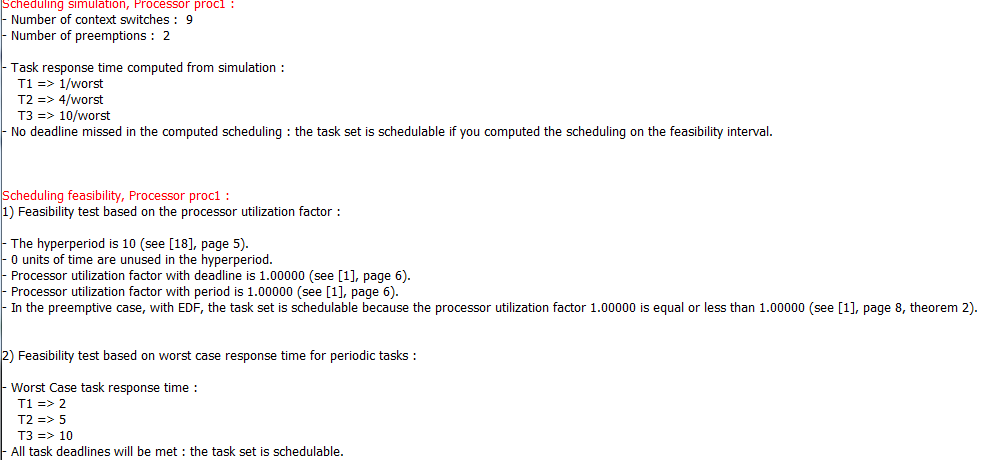
\includegraphics[width=0.8\textwidth]{5_EDF.png}
    \caption{Example 5 Earliest Deadline First}
\end{figure}

\subsubsection*{Example 6}
\begin{figure}[H]
    \centering
    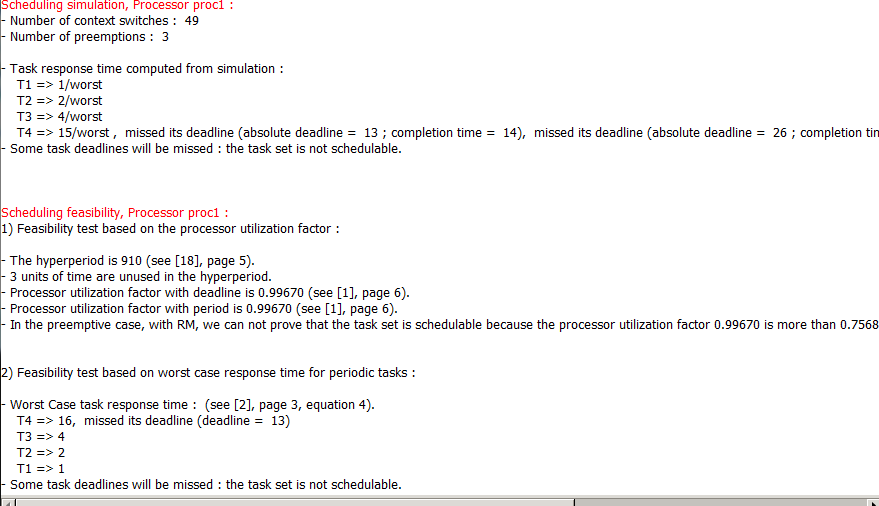
\includegraphics[width=0.8\textwidth]{6_RM.png}
    \caption{Example 6 Rate Monotonic}
\end{figure}
\begin{figure}[H]
    \centering
    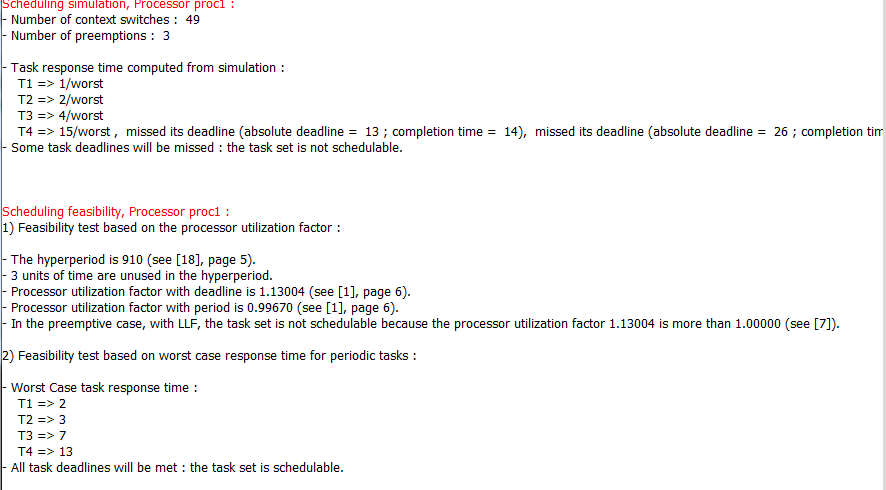
\includegraphics[width=0.8\textwidth]{6_LLF.png}
    \caption*{Example 6 Least Laxity First}
\end{figure}
\begin{figure}[H]
    \centering
    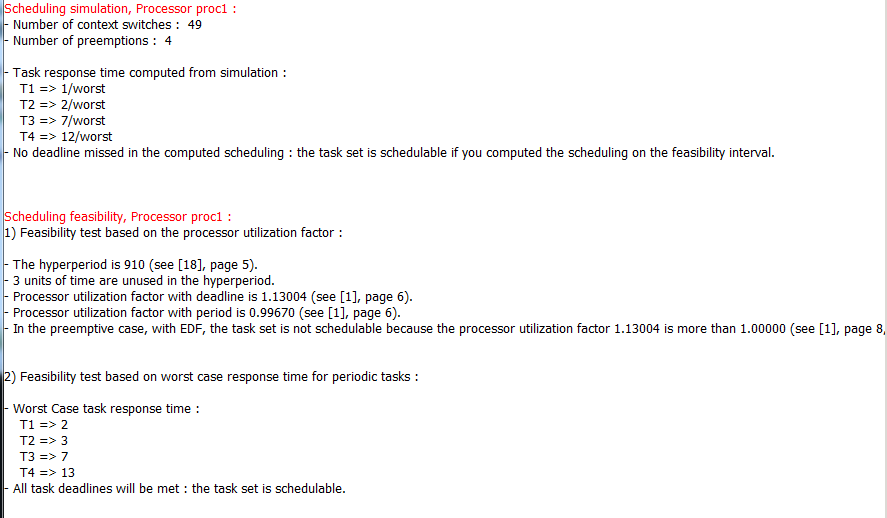
\includegraphics[width=0.8\textwidth]{6_EDF.png}
    \caption{Example 6 Earliest Deadline First}
\end{figure}

\subsubsection*{Example 7}
\begin{figure}[H]
    \centering
    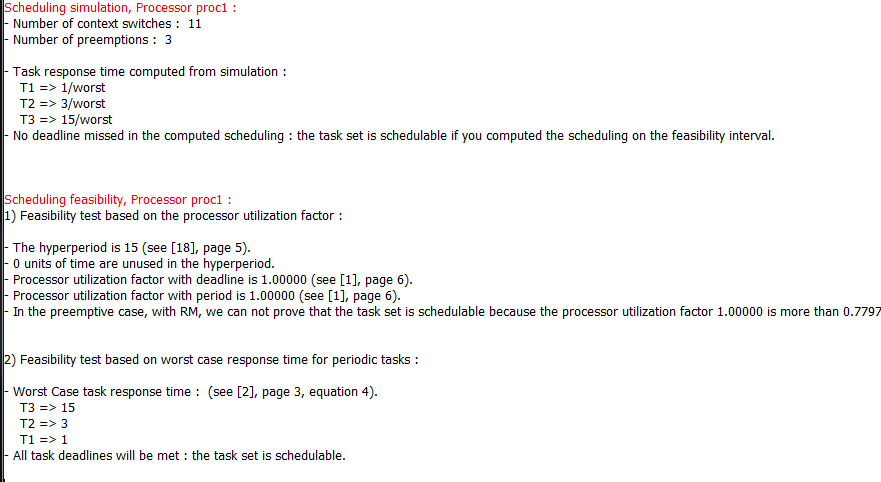
\includegraphics[width=0.8\textwidth]{7_RM.png}
    \caption{Example 7 Rate Monotonic}
\end{figure}
\begin{figure}[H]
    \centering
    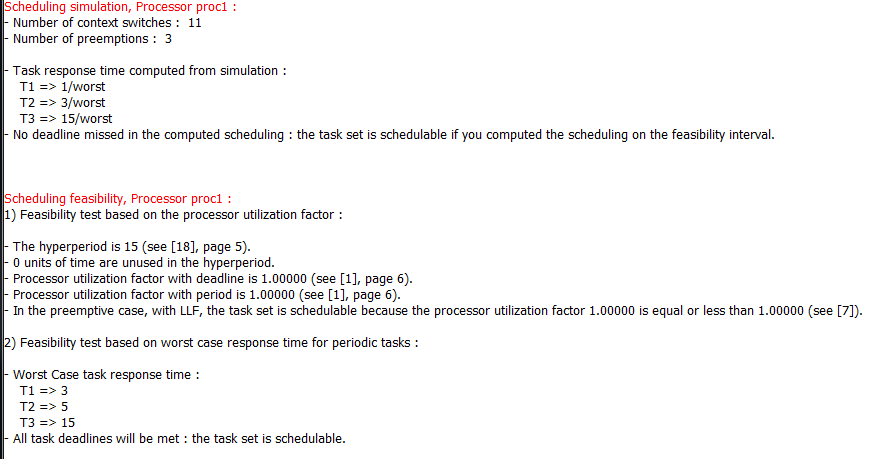
\includegraphics[width=0.8\textwidth]{7_LLF.png}
    \caption{Example 7 Least Laxity First}
\end{figure}
\begin{figure}[H]
    \centering
    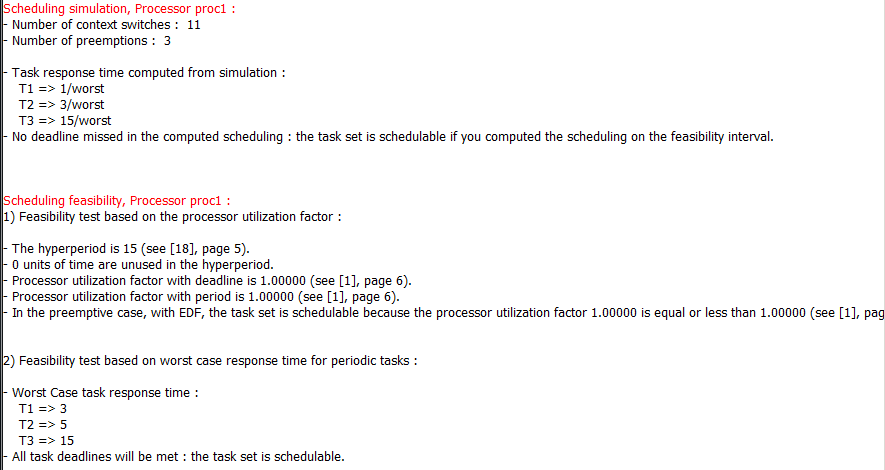
\includegraphics[width=0.8\textwidth]{7_EDF.png}
    \caption{Example 7 Earliest Deadline First}
\end{figure}

\subsubsection*{Example 8}
\begin{figure}[H]
    \centering
    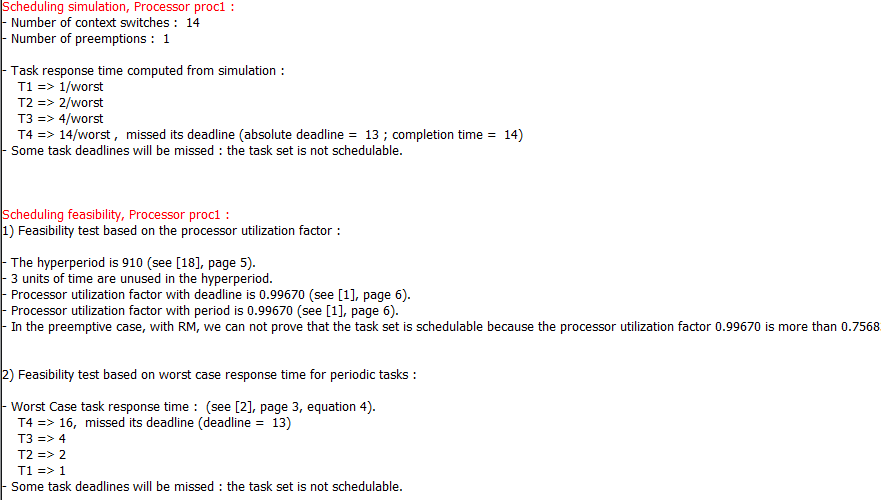
\includegraphics[width=0.8\textwidth]{8_RM.png}
    \caption{Example 8 Rate Monotonic}
\end{figure}
\begin{figure}[H]
    \centering
    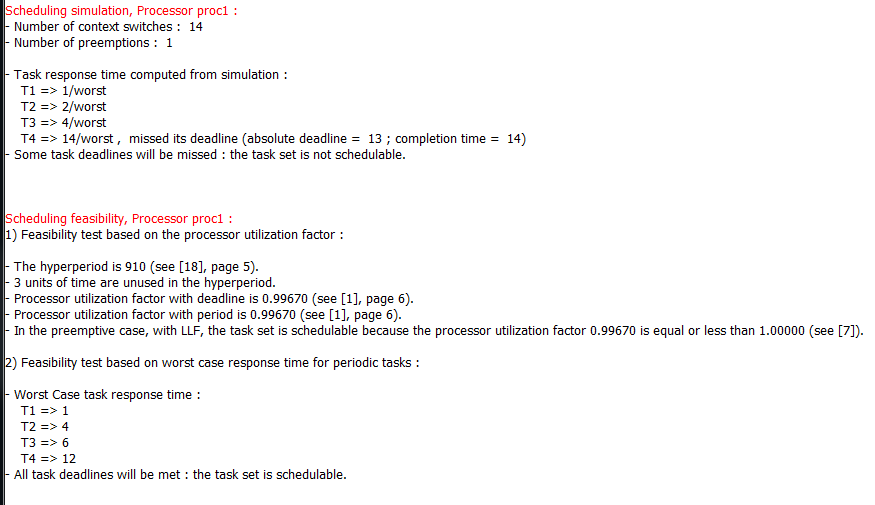
\includegraphics[width=0.8\textwidth]{8_LLF.png}
    \caption{Example 8 Least Laxity First}
\end{figure}
\begin{figure}[H]
    \centering
    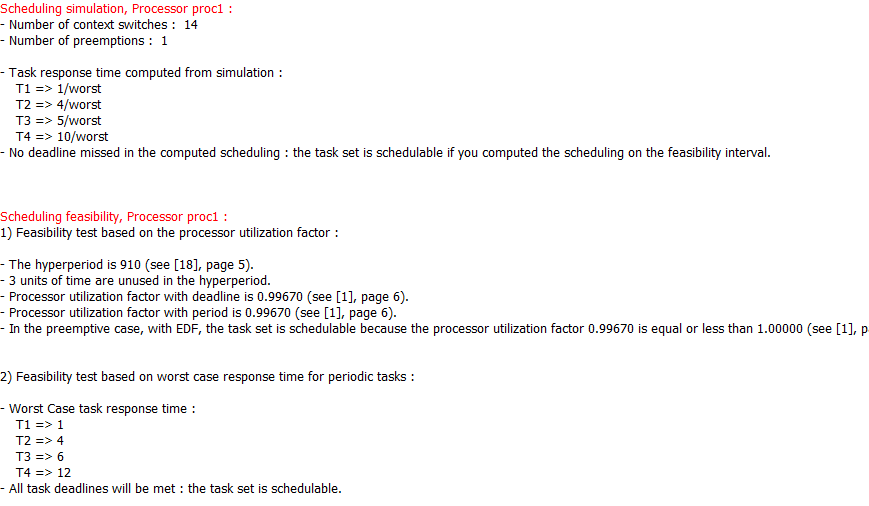
\includegraphics[width=0.8\textwidth]{8_EDF.png}
    \caption{Example 8 Earliest Deadline First}
\end{figure}

\section*{Problem 4}
\subsection*{Constraints}
\begin{itemize}
    \item The deadline of a system is equivalent to its period. 
    \item Fixed Priority, Preemptive, Run-to-Completion Scheduling is used
    \item The LUB must never pass a task set that will fail
\end{itemize}
\subsection*{Assumptions}
These are largely the same assumptions they make for the rate monotonic protocol.
\begin{itemize}
    \item The requests for all tasks with hard deadlines are periodic with constant interval between each request
    \item Each request must be capable of finishing within its period, this is known as the run-ability constraint
    \item Run-time is known and deterministic for these evaluations. 
\end{itemize}
\subsection*{Key steps}
The important thing to note about this derivation is that it starts with a set of rules that works under a very strict set of constraints and then works towards being more general. The major theorems that are used all try to generalize previous steps to a broader set of constraints.
\begin{itemize}
    \item One of the key steps for the LUB derivation is providing a priority assignment. This happens before the section on the derivation, but is essential to the proof because it provides an assignment of priorities. The proof for this is done on a set of two tasks, but the way it is done could be extended to infinitely many more.
    \item Another essential step is Theorem 3. It defines the least upper bound for a set of two tasks, this is important because it provides a mathematical basis for extending the bound to multiple tasks. It follows the idea that you can start simply and then add complexity as you go. The proof is also kind of "tricky" because it requires the analysis of two different cases that a two task system could be in. The two cases are when task 1 finishes quickly enough to not effect task 2's critical section and when it doesn't.
    \item Theorem 4 adds another level of complexity by extending the bound to m tasks, while adding in the restriction that the ratio between request periods is less than 2. I consider this interesting because the Liu and Layland used the ratio between periods to find an effective way to bridge the proof gap between Theorem 3 and Theorem 5. It is also nice that they use derivatives to find the minimum towards the end of that proof.
\end{itemize}

\end{document}
